\chapter{Results \label{chap:results}}

\section{Survey}
The survey was completed by 12 people in total. Half of the participants have described themselves as well-acquainted with the area of games or animation. One person was not sure and the rest was not acquainted with that topic. However it appears that this is never strongly correlated (using Pearson correlation coefficient) to any of the other answers. It seems that having experience in games or animation does not significantly influence how the participants perceived the animations.

The participants were asked to decide whether the animations presented to them were realistic. The question was asked about each of the six scenes. The t-test was performed taking into account the answers about all the original scenes and the recreated scenes. The p-value of 0.7614 shows weak statistical significance of the result. The realism of the scenes was described on a one to five scale\footnote{The participants were asked to say whether they agree with the statement  `video X is realistic'. The answer was taken on a one to five scale where one means `strongly agree' and five means `strongly disagree'}, where the average score for both original and recreated scenes is about 3.1. These results show that animations generated by this project are no more realistic than the originals and that both original and recreated scenes are hardly realistic at all.
	
A similar set of questions was asked about the effectiveness in conveying emotions. The participants were asked to decide whether the animations correctly convey the feelings and emotions of the characters in the scene. This time the results yielded the p-value of 0.4657 showing a higher significance of the result. The participants' answers suggest that the animations reproduced by the software are slightly better at conveying feelings and emotions (the mean score of the recreated animations was by 0.3 (out of 5) better than the originals). These results show a very slight advantage of the recreated animations over the original ones.

The figure ~\ref{fig:realism_graph} shows a breakdown of these results for each game. The graph shows that the software is capable of creating more realistic animation than animation featured in an old game, but struggles to keep up with newer titles. The recreated animations are on average considered more realistic than animation from a 2008 game. The software produces animations of similar realism as animations featured in a 2015 game and is slightly outperformed by a 2017 game. One thing that is worth noticing is that the data suggests that the recreated scenes are capable of conveying the emotions and feelings correctly, however this is not enough for them to be seen as `realistic'.

\begin{figure}[!ht]
	\centerline{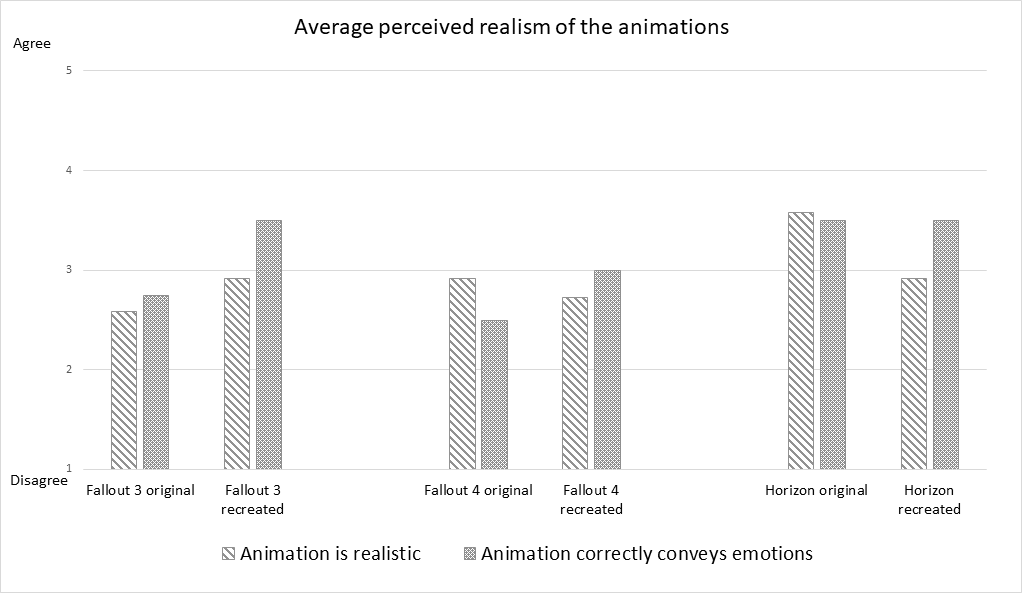
\includegraphics[width = 42em]{img/results/realism.png}}
	\caption{Average perceived realism of the animations}\label{fig:realism_graph}
\end{figure}



Despite the not so positive results above, the participants actually seem to prefer the recreated videos. When asked if the recreated animation makes the scene more enjoyable almost 70\% of participants agreed (figure ~\ref{fig:improves_graph}). Similarly, over 60\% of participants (figure ~\ref{fig:prefer_graph}) pointed to the recreated animation when asked which animation do they subjectively prefer. The interviewees justified their choice by statements such as `Body language matches with what is being said' or `More accurate expression of feelings'. Adversely, the supporters of the original animations described the recreated animation as `over the top' and with `weird hand movements'. The answers do not differ greatly game to game.

\begin{figure}[!ht]
	\centerline{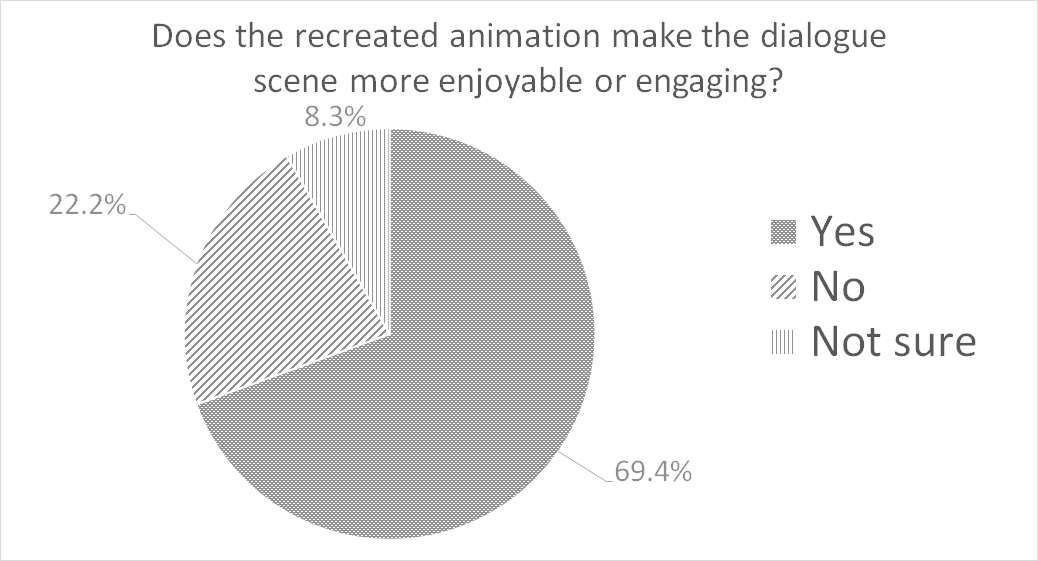
\includegraphics[width = 42em]{img/results/improves.png}}
	\caption{Does the recreated animation make the dialogue scene more enjoyable or engaging?}\label{fig:improves_graph}
\end{figure}

\begin{figure}[!ht]
\centerline{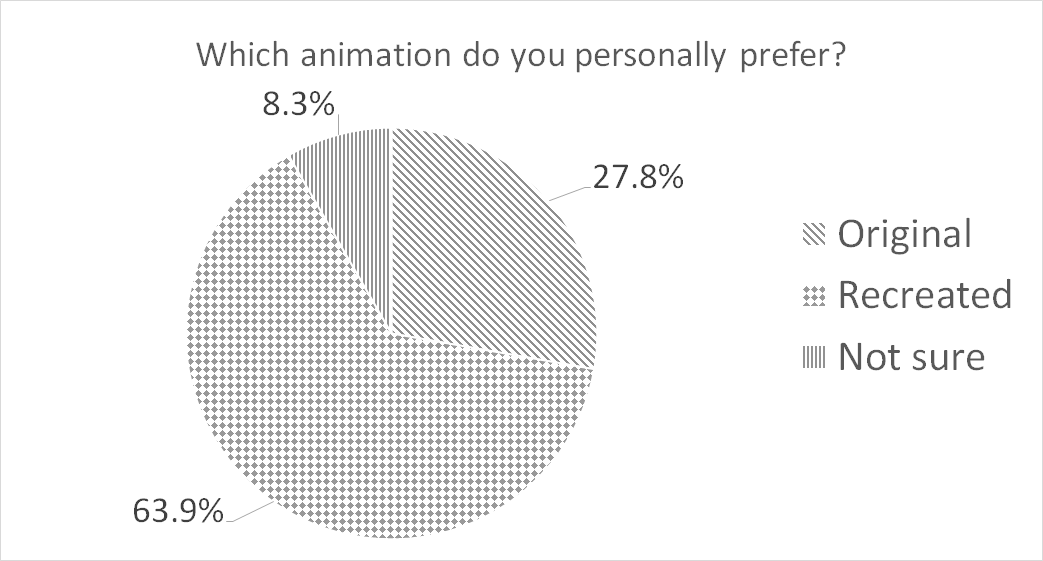
\includegraphics[width = 42em]{img/results/prefer.png}}
\caption{Which animation do you personally prefer?}\label{fig:prefer_graph}
\end{figure}


The last important piece of information gathered from the participants was whether they though that the animations generated by the software need adjustments before being used in a finished game. The answers lean slightly into the `needs serious adjustments' side, however the average suggests that the animations need a moderate amount of adjustments.

\begin{figure}[!ht]
	\centerline{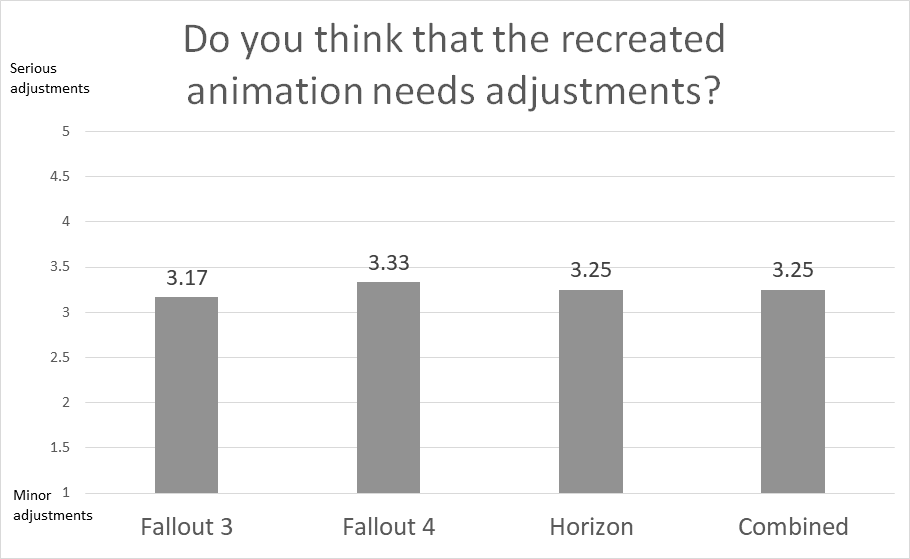
\includegraphics[width = 42em]{img/results/adjustments.png}}
	\caption{Do you think that the recreated animation needs adjustments (before being used in a finished game)?}\label{fig:adjustments_graph}
\end{figure}











